% !TeX program = lualatex
% !TeX encoding = UTF-8

\documentclass[a4paper,1pt,landscape]{article}

\usepackage{siunitx}
\usepackage[dvipsnames]{xcolor}
\usepackage{tikz}
\usetikzlibrary{decorations.pathmorphing}
\usepackage[hmargin=1cm,vmargin=1cm]{geometry}

\begin{document}
\centering
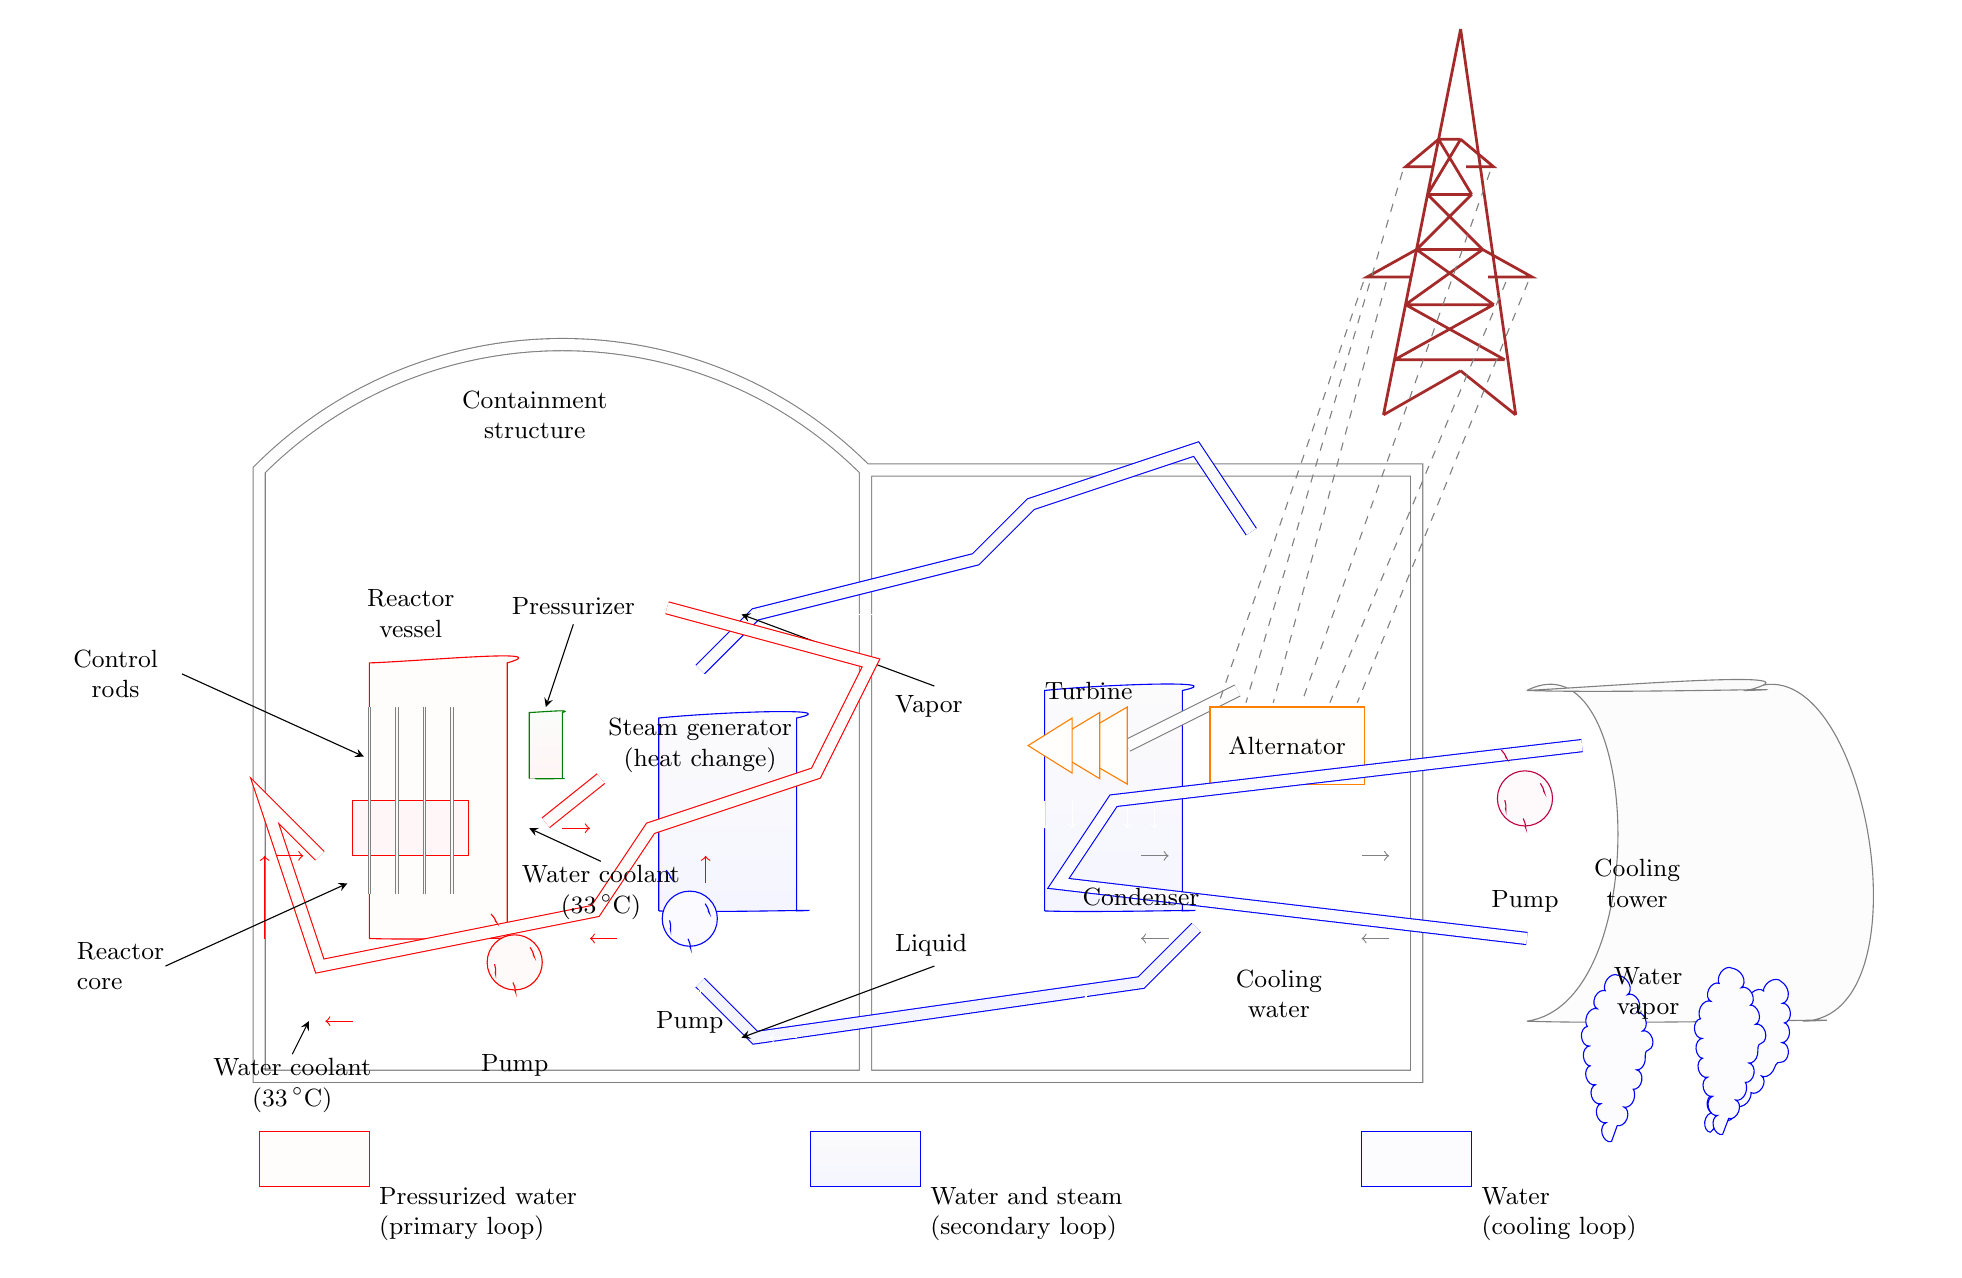
\begin{tikzpicture}[
		scale=.7,
		annotline/.style = {stealth-},
		arrows1loop/.style={->,red},
		arrows2loop/.style={->,white},
		arrows3loop/.style={->,draw=Gray},
	]
	\draw[draw=Gray,double=Gray!1,double distance=4pt]
	(12,12) to[out=135,in=45](,12)--(,)--(22,)--(22,12)--(12,12)--(12,);
	\node[text width=4cm, text centered,font=\small] at (6,13)
	{Containment\\structure};

	% legend
	\begin{scope}[yshift=-2cm]
		\filldraw[draw=red,fill=red!1] (1,) rectangle ++(2,1);
		\node[text width=4cm, font=\small,right] at (3,.5)
		{Pressurized water\\(primary loop)};
		\filldraw[draw=blue,bottom color=blue!4,top color=Gray!3]
		(11,) rectangle ++(2,1);
		\node[text width=4cm, font=\small,right] at (13,.5)
		{Water and steam\\(secondary loop)};
		\filldraw[draw=Blue,fill=Blue!1] (21,) rectangle ++(2,1);
		\node[text width=4cm, font=\small,right] at (23,.5)
		{Water\\(cooling loop)};
	\end{scope}

	% 2nd Loop
	\begin{scope}[xshift=7.25cm,yshift=3cm]
		% vessel left
		\filldraw[draw=blue,bottom color=blue!4,top color=Gray!3]
		(,) to[out=-2,in=2] (3.5,) --
		(3.5,4.5) to[out=12,in=6] (,4.5) -- (,);
		% vessel right
		\filldraw[draw=blue,bottom color=blue!4,top color=Gray!3,xshift=7cm]
		(,) to[out=-2,in=2] (3.5,) --
		(3.5,5) to[out=12,in=6] (,5) -- (,);
		% circuits
		\draw[draw=blue,double=blue!4,double distance=4pt]
		(1.75,-.3) -- ++(,-1) -- ++(7,) -- ++(,1);
		\draw[draw=blue,double=Gray!3,double distance=4pt]
		(1.75,5.38) -- ++(,1) -- ++(4,) -- ++(,1) -- ++(3,) -- ++(,-1.5);
		% arrows
		\draw[arrows2loop] (3.5,-1.3) -- (3,-1.3);
		\draw[arrows2loop] (1.75,-.9) -- (1.75,-.4);
		\draw[arrows2loop] (4.5,6.38) -- (5,6.38);
		\draw[arrows2loop] (7,7.38) -- (7.5,7.38);
		\draw[arrows2loop] (8.75,6.4) -- (8.75,5.9);
		\draw[arrows2loop] (8.75,-.4) -- (8.75,-.9);
		%
		\foreach \x in {.5,1,...,3}
		\draw[arrows2loop,xshift=7cm] (\x,3) -- (\x,2.5);
		% labels
		\draw[annotline] (2.5,-1.3) -- ++(3.5,1.3)
		node[text width=1cm,font=\small,above] {Liquid};
		\draw[annotline] (2.5,6.38) -- ++(3.5,-1.3)
		node[text width=1cm,font=\small,below] {Vapor};
		% pump
		\begin{scope}[xshift=16,yshift=-4]
			\filldraw[fill=Blue!2,draw=Blue] (,) circle (.5cm);
			\node[below,font=\small] at (,-.5) {Pump};
			\filldraw[fill=Blue!4,draw=Blue,yshift=-.5cm]
			(,) arc (24:18:.4cm)  arc (2:28:.4cm) ;
			\filldraw[fill=Blue!4,draw=Blue,yshift=+.5cm,rotate=18]
			(,) arc (24:18:.4cm)  arc (2:28:.4cm) ;
			\filldraw[fill=Blue!4,draw=Blue,xshift=+.5cm,rotate=9]
			(,) arc (24:18:.4cm)  arc (2:28:.4cm) ;
			\filldraw[fill=Blue!4,draw=Blue,xshift=-.5cm,rotate=-9]
			(,) arc (24:18:.4cm)  arc (2:28:.4cm) ;
		\end{scope}
		% generator ...
		\draw[xshift=6.5cm,draw=Gray,double=Gray!1,double distance=4pt]
		(3,4) -- ++(2,);
		\filldraw[xshift=6.5cm,fill=orange!1,draw=orange]
		(1.8,4) -- (3.,3.3) -- (3.,4.7) -- cycle;
		\filldraw[xshift=6.5cm,fill=orange!1,draw=orange]
		(1.5,4) -- (2.5,3.4) -- (2.5,4.6) -- cycle;
		\filldraw[xshift=6.5cm,fill=orange!1,draw=orange]
		(1.2,4) -- (2  ,3.5) -- (2  ,4.5) -- cycle;
		\filldraw[xshift=6.5cm,fill=orange!1,draw=orange]
		(4.5,3.3) rectangle (7.3,4.7);
		%labels
		\node[text width=3cm, text centered,font=\small] at (1.75,4)
		{Steam generator\\ (heat change)};
		\node[text width=2cm, text centered,font=\small] at (8.8,5) {Turbine};
		\node[text width=2cm, text centered,font=\small] at (12.4,4) {Alternator};
		% transmission lines
		\node (aa) at (11.1,4.6) {};
		\node (bb) at (11.6,4.6) {};
		\node (cc) at (12.1,4.6) {};
		\node (dd) at (12.6,4.6) {};
		\node (ee) at (13.1,4.6) {};
		\node (ff) at (13.6,4.6) {};

	\end{scope}

	% 3 Loop
	\begin{scope}[xshift=23cm,yshift=1cm]
		% circuit
		\draw[draw=Blue,double=Blue!1,double distance=4pt]
		(1,2.5) -- ++(-8.5,) -- ++(,+1.5) -- ++(8.5,);
		% arrows
		\draw[arrows3loop] (-5.5,2.5) -- (-6,2.5);
		\draw[arrows3loop] (-1.5,2.5) -- (-2,2.5);
		\draw[arrows3loop] (-6,4) -- (-5.5,4);
		\draw[arrows3loop] (-2,4) -- (-1.5,4);
		% tower
		\filldraw[draw=Gray,fill=Gray!2] (1,7) to[out=27,in=8]
		(,) to[out=-2,in=2]
		(6,) to[out=1,in=27]
		(5,7);
		\filldraw[draw=Gray,fill=Gray!4] (1,7) to[out=3,in=15]
		(5,7) to[out=2,in=-2]
		(1,7);
		% labels
		\node[text width=3cm, text centered,font=\small] at (3,3.5)
		{Cooling\\tower};
		\node[text width=2cm, text centered,font=\small] at (-3.5,1.5)
		{Cooling\\water};
		\node[text width=2cm, text centered,font=\small] at (-6,3.25)
		{Condenser};
		% pump
		\begin{scope}[xshift=-1,yshift=115]
			\filldraw[fill=purple!2,draw=purple] (,) circle (.5cm);
			\node[below,font=\small] at (,-.5) {Pump};
			\filldraw[fill=purple!4,draw=purple,yshift=-.5cm]
			(,) arc (24:18:.4cm)  arc (2:28:.4cm) ;
			\filldraw[fill=purple!4,draw=purple,yshift=+.5cm,rotate=18]
			(,) arc (24:18:.4cm)  arc (2:28:.4cm) ;
			\filldraw[fill=purple!4,draw=purple,xshift=+.5cm,rotate=9]
			(,) arc (24:18:.4cm)  arc (2:28:.4cm) ;
			\filldraw[fill=purple!4,draw=purple,xshift=-.5cm,rotate=-9]
			(,) arc (24:18:.4cm)  arc (2:28:.4cm) ;
		\end{scope}
	\end{scope}

	% Loop
	\begin{scope}[xshift=2cm,yshift=4cm]
		% Reactor vessel
		\filldraw[draw=red,fill=red!1] (,-.5) to[out=-2,in=2]
		(3.5,-.5) --
		(3.5,4.5) to[out=16,in=2]
		(,4.5) --
		(,-.5);

		% circuit
		\draw[draw=red,double=red!1,double distance=4pt]
		(.1,1) --  ++(-1,) -- ++(,-3) -- ++(5,) -- ++(,1.5) --
		++(3,) -- ++(,2) -- ++(-3.7,);

		% Pressurizer
		\draw[draw=red,double=red!1,double distance=4pt] (4.2,1.6) -- ++(,.8);
		\filldraw[draw=Green,bottom color=red!4,top color=Green!2]
		(4,2.4) to[out=-2,in=2]
		(4.5,2.4) --
		(4.5,3.6) to[out=16,in=2]
		(3.9,3.6) --
		(3.9,2.4);

		% arrows
		\draw[arrows1loop] (-.7,1) -- (-.2,1);
		\draw[arrows1loop] (-.9,-.5) -- (-.9,);
		\draw[arrows1loop] (.7,-2) -- (.2,-2);
		\draw[arrows1loop] (4.5,1.5) -- (5,1.5);
		\draw[arrows1loop] (7.1,.5) -- (7.1,);
		\draw[arrows1loop] (5.5,-.5) -- (5,-.5);

		% pump
		\begin{scope}[xshift=75,yshift=-55,fill=red!2,draw=red]
			\filldraw (,) circle (.5cm);
			\node[below,font=\small] at (,-.5) {Pump};
			\filldraw[yshift=-.5cm] (,) arc (24:18:.4cm)  arc (2:28:.4cm) ;
			\filldraw[yshift=+.5cm,rotate=18]
			(,) arc (24:18:.4cm)  arc (2:28:.4cm) ;
			\filldraw[xshift=+.5cm,rotate=9]
			(,) arc (24:18:.4cm)  arc (2:28:.4cm) ;
			\filldraw[xshift=-.5cm,rotate=-9]
			(,) arc (24:18:.4cm)  arc (2:28:.4cm) ;
		\end{scope}

		% reactor core
		\filldraw[fill=red!3,draw=red] (.7,) rectangle (2.8,2);

		% control rods
		\foreach \x in {1.,1.5,2.,2.5}
		\draw[draw=Gray,double=Gray!5,double distance=.5pt] (\x,.3) -- (\x,3.7);

		%labels
		\draw[annotline] (.6,.5) -- ++(-3.3,-1.5)
		node[text width=1cm,font=\small,left] {Reactor core};
		\node[text width=2cm, text centered,font=\small] at (1.75,5.4)
		{Reactor vessel};
		\draw[annotline] (.9,2.8) -- ++(-3.3,1.5)
		node[text width=2cm, text centered,font=\small,left=-8pt] {Control\\rods};
		\draw[annotline] (4.2,3.7) -- ++(.5,1.5)
		node[text width=2cm, text centered,font=\small,above] {Pressurizer};
		\draw[annotline] (3.9,1.5) -- ++(1.3,-.6)
		node[text width=2.4cm, text centered,below=-2pt,font=\small]
		{Water coolant (\qty{33}{\degreeCelsius})};
		\draw[annotline] (-.1,-2) -- ++(-.3,-.6)
		node[text width=2.4cm, text centered,below=-2pt,font=\small]
		{Water coolant (\qty{33}{\degreeCelsius})};
	\end{scope}

	% clouds
	\begin{scope}[xshift=26cm,yshift=1cm, fill=blue!1, draw=Blue,
		decoration={bumps,segment length=.5cm}]
		\filldraw[yshift=-1.5cm,rotate=-25,decorate]
		(,) -- ++(-.4,1.25)-- ++(-.1,.75)-- ++(.2,.5)-- ++(.3,.5)--
		++(.3,-.5)-- ++(.2,-.5)-- ++(-.1,-.75)-- ++(-.4,-1.25);
		\filldraw[xshift=.5cm,yshift=-2cm,rotate=-3,decorate]
		(,) -- ++(-.4,1.25)-- ++(-.1,.75)-- ++(.2,.5)-- ++(.3,.5)--
		++(.3,-.5)-- ++(.2,-.5)-- ++(-.1,-.75)-- ++(-.4,-1.25);
		\filldraw[xshift=-1.5cm,yshift=-2.15cm,rotate=-2,decorate]
		(,) -- ++(-.4,1.25)-- ++(-.1,.75)-- ++(.2,.5)-- ++(.3,.5)--
		++(.3,-.5)-- ++(.2,-.5)-- ++(-.1,-.75)-- ++(-.4,-1.25);
		%labels
		\node[text width=1cm, text centered,font=\small] at (.2,1.5) {Water vapor};
	\end{scope}

	% palo della luce
	\begin{scope}[xscale=.2,xshift=113cm,yshift=19cm,line width=1pt,Brown]
		\draw (,) -- (-6,-6)
		(,) -- ( 6,-6)
		(-1,-1) -- ( 1,-1)
		(-1,-1) -- ( 2,-2)
		( 1,-1) -- (-2,-2)
		(-2,-2) -- ( 2,-2)
		(-2,-2) -- ( 3,-3)
		( 2,-2) -- (-3,-3)
		( 3,-3) -- (-3,-3)
		(-3,-3) -- ( 4,-4)
		( 3,-3) -- (-4,-4)
		( 4,-4) -- (-4,-4)
		(-4,-4) -- ( 5,-5)
		( 4,-4) -- (-5,-5)
		( 5,-5) -- (-5,-5)
		(-6,-6) -- ( ,-5.2)
		( 6,-6) -- ( ,-5.2);
		\draw (-1.5,-1.5) -- (-4,-1.5) -- (-1,-1)
		( 1.5,-1.5) -- ( 4,-1.5) -- ( 1,-1);
		\path (-4,-1.4) node (a) {}
		( 4,-1.4) node (b) {};
		\draw[line width=1pt,Brown] (-3.5,-3.5) -- (-7.5,-3.5) -- (-3,-3)
		( 3.5,-3.5) -- ( 7.5,-3.5) -- ( 3,-3);
		\path (-7.5,-3.4) node (c) {}
		( 7.5,-3.4) node (d) {}
		(-5.5,-3.4) node (e) {}
		( 5.5,-3.4) node (f) {};
	\end{scope}

	% transmission lines
	\draw[dashed,Gray] (c) -- (aa)
	(a) -- (bb)
	(e) -- (cc)
	(b) -- (dd)
	(f) -- (ee)
	(d) -- (ff);
\end{tikzpicture}

\end{document}
